\documentclass[stu]{apa7}
\usepackage[utf8]{inputenc}
\usepackage[english]{babel}
\usepackage{csquotes}
\usepackage{lipsum}
\usepackage{amsmath}

%\usepackage{tocloft}
%\renewcommand{\cftsecleader}{\cftdotfill{\cftdotsep}}

\setlength{\parindent}{0.5in}

\usepackage{hyperref}
\hypersetup{
	colorlinks=true,
	linkcolor=black,
	citecolor=black,
	urlcolor=cyan
}

\usepackage{enumitem}
\setlist{noitemsep}

%\usepackage{geometry}
%\geometry{
%	top=25mm,
%	bottom=25mm,
%	left=25mm,
%	right=25mm
%}

\usepackage[style=apa, doi=false, backend=biber, natbib]{biblatex}
\addbibresource{ref.bib}
\AtEveryBibitem{
	\clearfield{url}
	\clearfield{urldate}
	\clearfield{note}
	\clearfield{annote}
}

\usepackage{graphicx}
% \bibliographystyle{elsarticle-num}

%\title{}
%\shorttitle{}


\begin{document}

%\begin{center}
	\uppercase{National Research University Higher School of Economics}\\
	\textbf{Saint Petersburg School of Economics and Management}\\
	\textbf{Department of Economics}
\end{center}

\vspace{4\baselineskip}

\begin{center}
	Project Proposal\\
	\textbf{Forecasting Russian Financial Time Series Using Deep Learning Methods}
\end{center}

\vspace{2\baselineskip}

\begin{flushright}
	Yuriy A. Sosnin\\
	BEC-182\\

	\vspace{\baselineskip}

	Academic Supervisor:\\
	Vladimir N. Pyrlik\\
	Associate Professor
\end{flushright}

\vspace{\fill}

\begin{center}
	Saint Petersburg

	2022
\end{center}

\thispagestyle{empty}

\clearpage


\tableofcontents
\clearpage

\section{Abstract}

This purpose of this study is to investigate the relationship between a list of macroeconomic variables and quality with which Deep Learning can predict Russian stock market. The connection between commodity prices, exchange rates, inflation, and foreign markets is a well-established area of economic and econometric research. On the other hand, in the prediction field, while modern Deep Learning methods are becoming more and more popular for financial time series forecasting, those fundamental economic factors are rarely utilized.
Using daily data on several Russian publicly traded companies in the period of 2011-2019, I plan to determine if the mentioned factors are suitable as inputs for LSTM model, improving its performance compared to baselines and ARIMA in terms of RMSE.

\section{Introduction}

% Intro?

In recent years, the surge in the power of Machine Learning, and especially Deep Learning, has lead to dramatic advancements in computer vision, natural language processing, and various other tasks, including time series forecasting, and, in particular, financial time series forecasting \citep{lara-benitez_experimental_2021}.
However, this stream of literature is inherently technical.
Machine Learning specialists view financial data merely as one of time series domains, alongside fields like energy consumption, weather forecasting or turnout rates.
Their works, while contributing to minimizing prediction error, use little knowledge of economics or finance to provide any meaningful insights of the way financial markets work of behave.
The series considered are either univariate, use standard High-Low-Open-Close data on stocks, or other ML-suitable data like tweets or news articles \citep{sezer_financial_2019}.
Macroeconomic factors such as exchange rates or oil prices can hardly be found.

On the other hand, economists searching for causality between stock markets and fundamental factors based on theoretical insights is a different stream of literature. Connections of stock markets with oil prices, exchange rates, inflation and foreign markets have been documented for countries around the world \citep{verma_impact_2021}. However, these works use different, statistical toolkit, consisting of mostly linear and ARCH methods. In terms of pure prediction power, Machine Learning methods like Random Forest or SVM are proved to produce better results than linear Box-Jenkins approaches \citep{kumar_forecasting_2006}. Deep learning approaches like LSTM outperform them as well \citep{siami-namini_forecasting_2018}.

% Russia?

My aim therefore is to test applicability of macroeconomic data for the task of forecasting Russian stock prices time series. Compared to univariate setting, do factors like oil prices, exchange rates or foreign market indexes improve predictions produces by Deep Learning algorithms?

It is not a classic econometric study, as improving prediction does not imply causality. However, improving prediction would mean there is certainly some relevant information, which powerful ML methods are able to retrieve and utilize.

\subsection{Financial Time Series Foracasting}



\subsection{Forecasting models}

Econometric models employed by authors in most of mentioned articles are either some variations of GARCH (generalized autoregressive conditional heteroskedasticity) model or VAR, a multivariate generalization of ARIMA (autoregressive integrated moving average) model. While being suitable for causality determination, in terms of predictive power, those are by far not the state of the art at the moment \citep{siami-namini_forecasting_2018}. It is apparent that for as complex entity as stock market prices or returns <<simple>> linear or ARCH models do not suffice.

Deep Learning has gained popularity with remarkable increase of its power, complexity and number of possible applications. Financial time series is no exception. An increasing number of articles are being published by ML specialists, introducing new models and approaches. I will cover the basic and most popular architectures.

The basic deep learning architecture is Artificial Neural Network \citep{sezer_financial_2019}. It is, broadly speaking, a combination of parametric matrix multiplications with non-linear activation function applied to each of them, stacked together. For each vector of variables (in time series context, lags of the variable of interest) a single value $y_{t+1}$ is produced. Then, it is compared with the true future value using a loss function. Because loss functions and all layer operations are differentiable with respect to parameters, gradients can be calculated, and the parameters get updated in the direction of minimizing the loss, with a procedure called backpropagation. After sufficient number of iterations, the model <<learns>> the best parameters.

The simple ANN model, however, is somewhat equivalent to running a linear regression on lagged time series data: it does not account for time dependence and autocorrelation \citep{torres_deep_2021}. For this purpose, Recurrent Neural Networks were introduced, first in the field of Natural Language Processing \citep{hewamalage_recurrent_2021}. An RNN is made of a single <<cell>> (still a combination of parametric matrix multiplication, concatenation and nonlinear functions) rolling over instances of a time-dependent data. In this architecture an input is a sequence of some predefined length, and the model gets applied to every sequence in the data in a rolling window manner.

There are several types of RNN cells, each carefully designed by ML researches to better accomplish prediction tasks. The most widely used is called LSTM, Long Short-Term Memory \citep{greff_lstm_2017}.
Initially designed to deal with the vanishing gradient problem, LSTM can also utilize both short- and long-term temporal dependence by receiving previous step state as input, which makes it very good for time series tasks with autocorrelation of higher orders.

Most of papers in this field employ DL architectures in single-stock forecasting task. A number of basic variables like Open, Close prices, Volume and Volatility of a stock or a stock index are fed into a neural network of some new design, then the results are compared to previously developed models and baselines. % (for example, x, y, z).
Some of the authors use technical indicators \citep[e.g.][]{nelson_stock_2017, chen_lstm-based_2015}. % include other OR reviews because there is as ton of them
There is a stream of literature incorporating complex information like tweets, news or Google trends into forecasting framework, using different specific NN architectures for processing that data \citep{huang_using_2020, kordonis_stock_2016, hu_predicting_2018}. Some just use a very large number of stocks at the same time for training \citep{li_stock_2018}.

However, meaningful external macroeconomic factors are rarely used.
The closest work in some sense is by \citet{chen_constructing_2021}. The authors test, whether information on gold and oil prices is suitable for predicting future stock movement (a classification task, contrary to regression task of predicting the future value), using a Convolution Neural Network (CNN). They conclude that this external information enhance forecasts for firms from semiconductor, petroleum, and automotive industries, while not affecting apparel, fast food, and copy processing industries.
I plan a somewhat similar approach.

\subsection{Macroeconomic Variables}

Among the most studied relationships of external variables with stock prices are oil prices, exchange rates and inflation. They make up a significant branch of financial econometric literature.

The link between oil prices and economic activity, and, hence, stock prices can be considered common knowledge. There are various theoretical explanations for this relationship \citep{degiannakis_oil_2018}.
Firstly, oil prices directly affect future cash flows of oil-producer and oil-consumer firms, which get evaluated in their stock price. Therefore, oil-producer stocks move in the same direction as oil price as it affects their profits, while oil-consumers experience a rise or reduction in their costs which should drive their stock's price to the opposite direction \citep{basher_oil_2006, filis_dynamic_2011}.
Secondly, oil prices affect basic macroeconomic variables such as output and inflation, which in turn have their effect on the whole financial market.
Finally, fluctuations in oil price increase uncertainty \citep{brown_energy_2002}.

As for empirical proofs, the situation in unclear.
For example, \citet{basher_oil_2012} and \citet{filis_macro_2010} find negative relationship, \citet{narayan_modelling_2010} document positive effect, and studies like \citet{silvapulle_nonparametric_2017} or \citet{zhu_modelling_2014} report no effect at all.
Moreover, it is apparent that different countries exhibit different effects from oil prices. The studies of \citet{mohanty_oil_2011} and \citet{wang_oil_2013} show that for oil-exporting countries the effect of oil price change is positive, and the opposite is true for oil-importing countries.
The same can be said about different sectors. Energy-supplying sectors have been found to be affected positively by oil prices, while energy-consumers such as Buildings, Manufacturing, Transport, Food, Chemical, Medical, Computer and other sectors are more likely to suffer from them \citep{narayan_new_2011, elyasiani_oil_2011}.

Another factor considered to be affecting stock prices is exchange rate. Economic reasoning is the following. Similar to oil prices, exchange rates affect future cash flows of exporting and importing firms \citep{bahmani-oskooee_relation_2015}. Depreciation of domestic currency benefits exporters, increasing their profits, and hurts importers, increasing their costs, and, through this, affects their stock prices. However, the reverse link is known as well: as the rise (or fall) in stock prices indicates rise (or fall) in their holders' wealth, it also affects demand for imports, driving exchange rate up (or down).

Empirical evidence here is even more ambiguous than for oil prices.
A number of studies document existence of relationship only for a subsample of studies countries \citep[][among many others]{inci_dynamic_2014, chen_untangling_2012}.
The direction and existence of causality also depends on market condition, flowing from  stock prices to exchange rates in crisis and from exchange rates to stock prices otherwise \citep{kollias_nexus_2012, tsagkanos_long-run_2013}.

There is also evidence of inflation \citep{anari_stock_2001, eldomiaty_associations_2019}, interest rates \citep{hashemzadeh_stock_1988}, real output \citep{durai_stock_2009, zhao_stock_1999}, commodity prices other than oil \citep{raza_asymmetric_2016, sadorsky_modeling_2014} and many other factors influencing stock market causally.

As for the case of Russia, there are studies examining causal determinants of Russian stock market. \citet{kordonis_stock_2016} consider the period between 1997 and 2012 and oil prices and eastern European stock markets performance as variables to affect stock market in Russia. According to their findings, oil prices stopped being significant after 2006, while correlation with other markets increased in that period. \citet{robert_d_gay_effect_2008} studies several emerging economies' markets, including Brazil, India, China and Russia in the period of 1999-2006. They report a not significant result for both oil prices and exchange rates and all four countries. \citet{lozinskaia_fundamental_2019} study the impact of oil prices, exchange rates, foreign stock indexes and interest rates on Russian stock market from 2003 to 2018. The authors document a varying relationship, with variations caused by structural breaks. This list of studies is by no means inclusive.

\section{Data and Methodology}

\subsection{Variable Description}

The target variable if the study is Moscow Exchange Index (IMOEX), russian benchmark capitalization-weighted composite index, calculated on 50 best-performing russian issuers of most important sectors of russian economy. As a benchmark index, it represents, broadly, the aggregated dynamics of Russian stock market, so forecasting it yields yada yada

I use daily data on IMOEX as well as a number of explanatory variables to perform the forecasts. The variables are:

\begin{itemize}
\item RTSI, the same index, but evaluated in USD instead of Rubles.
\item Moscow Exchange secotral indexes, namely MOEXOG, MOEXEU, MOEXTL, MOEXMM, MOEXFN, MOEXC, MOEXCH
\item Shares of top-10 IMOEX constitutes by capitalization
\item Euro and USD to Ruble exchange rates
\item Commodity prices of Oil, Natural Gas, and Gold
\item Foreign market indexes, London exchange index (FTSE), S\&P-500 and NASDAQ index
\item Yields of Russian government bonds, 1 week to 20 years maturity
\end{itemize}

For each vairable with standatd OCHLV set (Open, Close, High, Low prices, and trading Volume), 5 stationary features are calculated:

\begin{itemize}
\item Return

\begin{equation}
R_t = \frac{P^{Close}_t - P^{Close}_{t-1}}{P^{Close}_{t-1}}
\end{equation}

\item Range, relative difference betweed Hign and Low

\begin{equation}
Range_t = \frac{P^{High}_t - P^{Low}_{t}}{P^{Low}_{t}}
\end{equation}

\item Volatility, daily realized volatility calculated on 5-minute interval data

\begin{equation}
RV_t =
\end{equation}

\item Volume, total daily volume
\end{itemize}

The chosen period is from 2018-07-04 to 2019-11-01. This specific period is relatively stable and quiet, without evident structural breaks or extreme news that would undermine performance of the models. Forecasting extreme events, though being another research stream, is outside the scope of this study.

\subsection{Exploratory Data Analysis and Descriptive Statistics}

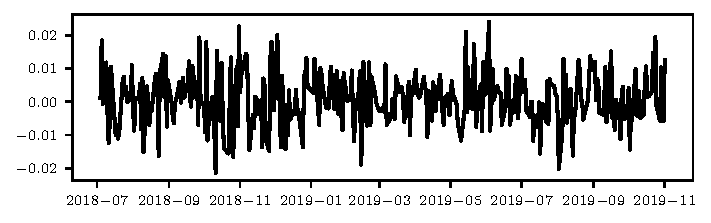
\includegraphics[width=\textwidth]{series.png}

\subsection{Modeling Technique}

Modeling task is multivariate rolling-window one-step-ahead regression forecasting, i.e. predicting one future value based on historical series of pre-defined fixed length. The data is reshaped to match inputs of deep learning models, which is a tensor on shape [B, L, N], where B is batch size, L is sequence length and N is a number of variables. Therefore, one input of a model is a tensor of stacked matrices of the following form:

\begin{equation}
input = \begin{bmatrix}
		y^{t} & x_{1}^{t} & \dots & x_{n}^{t} \\[1ex]
		y^{t-1} & x_{1}^{t-1} & \dots & x_{n}^{t-1} \\[1ex]
		y^{t-2} & x_{1}^{t-2} & \dots & x_{n}^{t-2} \\[1ex]
		\vdots & \vdots & \ddots & \vdots \\[1ex]
		y^{t-T} & x_{1}^{t-T} & \dots & x_{n}^{t-T}
\end{bmatrix}
\end{equation}

\begin{equation}
output = y^{t+1}
\end{equation}

The length of historic sequence considered at each step is a hyperparameter, and is chosen based on intuition and validaton performance. In my empirical experiments, it is set to either 10 or 20, two or four weeks history.

Before feeding into a model, the data is normalized, i.e. each variable is de-meaned and divided by its standard deviation. The scaling parameters are calculated only on training subset and applied to validation and test periods, to avoid information leakage.

Loss Functional, optimized by Gradient Decent algiriuthms of Neural Network models is Mean Squared Error, a sipmle and typical loss for regression problems. Forecasts are evaluated using MSE and Mean Directional Accuracy (MDA) metrics.

\begin{equation}
MSE = \frac{1}{N} \sum (y_t - \hat{y}_t)^2
\end{equation}

\begin{equation}
MDA = \frac{1}{N} \sum [ sign(\hat{y}_t)=sign(y_t) ]
\end{equation}

MSE directly measures squared deivation from the true value, making it the main metric for evaluating the performance of considered models. Directional accuracy is a simpler metic, evaluating only the correctness of predicted trend; it is used as an additional way to assess the quality of the models. Usage of this metric, should not be confused with *classification problem*, where only directions are forecasted in th e first place, and models are specifically taught to predict classes via Cross Entropy loss functional.

All models are trained using Adaptive Momentum Stochastic Gradient Decent optimization algorithm (ADAM).

\subsection{Validation Procedure}

Walk-Forward Cross Validation is employed as validation scheme. It is a common methodology in time series forecasting, thought underutilized in machine learning environment.

The data is sequentially split into 12 folds, one for each subsequent week of testing data. Each fold consists of 265 training instances, followed by validation and test preionds, 5 days (a trading week) each. For each fold, the training period is used to train model parameters, validation period is used to determine hyperparameters, and test period is used for final evaluation and comparison between different models.

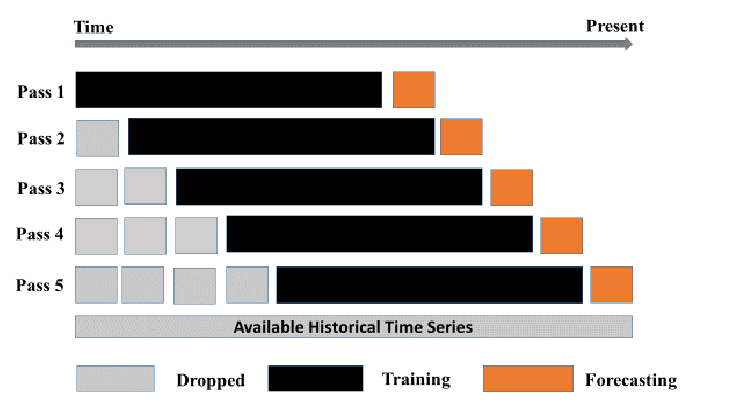
\includegraphics[width=\textwidth]{walkforward.png}

In contrast with dynamic or multiple-days-ahead forecasts, true values are input into the model for every subsequent day of the test period.

\subsection{Considered Models}

Baseline

LSTM

CNN-LSTM

CNN (?)

\section{Empirical Results}

The result of the study, firstly, is a choice of a best-performing model, in terms of RMSE. It is likely going to be LSTM or some variation of it, though it is not certain, hence the application of other models for comparison is planned. Researches have established that Neural Network approaches generally achieve higher quality predictions compared to linear models like ARIMA \citep{siami-namini_comparison_2018}. However, sometimes it does not hold for various reasons, like the choice of hyperparameters, suboptimal training procedure or the nature of the data. As training and testing the models on Russian stock has not been done previously, this study can provide an additional example of successful or unsuccessful application of DL in finance.

The other planned result is an interpretation of importance of suggested variables. In principle, the hypothesis for all of them is that they do bear significant information about stock market, and therefore must increase prediction quality. As reviewed literature suggest, most of the factors even have direct causal connection with the variable of interest. However, this does not imply that the variables will be important in this paper's setting. Determining it can motivate researches to use them in their works.

\section{Conclusion}

In the proposed study I plan to assess whether a list of different macroeconomic variables can increase quality of predictions on Russian stock market using Deep Learning models. As literature suggests, variables like oil prices, exchange rates, interest rates, foreign market indexes, and others can causally interact with stock prices of Russian companies. However, most of the variables have never been used outside of standard econometric pipelines, and modern Deep Learning models have not been exposed to that kind of information.

Therefore, training DL models on daily time series of Russian stock prices together with supplementary fundamental economic factors, this study aims to determine if those variables are applicable to the task of stock forecasting.
It can further strengthen or weaken the hypotheses about their links with the stock market, though not prove of disprove them. The proposed study is not a causal study; improving prediction power does not directly mean that a variable is causally significant, the opposite is not true as well.

Moreover, the results on Russia most likely will not be applicable to other countries or the future Russian stock market. Huge structural shocks can very drastically change the nature of stock markets and disrupt links between factors, rendering analysis inapplicable. However, this provides opportunity for future research to expand proposed methodology on other countries and different periods.

\printbibliography
% \bibliography{ref.bib}

\end{document}
